\section{Introduction}\label{sec:intro}
Audio deepfake detectors are used to flag speech that may have been synthesized or voice converted. In an authentication workflow, a false alarm can divert a bona fide recording to manual review, whereas a missed spoof can leave impersonation undetected. The cost of either decision depends on the workflow and the prevalence of spoofed traffic. A detector chosen by aggregate discrimination alone can behave differently at a fixed operating point after a recording passes through ordinary signal processing.

Noise and lossy coding are particularly relevant because they can occur in either order. Speech recorded in a noisy room may be encoded before transmission, while background audio can also be introduced after decoding. These pipelines preserve the intended class of a source, but change the evidence presented to a detector. Even with identical noise and codec settings, reversing the operators can change the waveform, spectral features, ranking, and fixed-threshold decisions. Measurements across matched views can isolate the influence of the implemented signal-processing order within a recorded source.

The accepted LAVA conference manuscript benchmarks six heterogeneous detectors. The extension presented here addresses a different question through a matched intervention on one detector architecture. Within each of two initialization blocks, the training recordings, order, optimizer, numerical backend, and checkpoint rule are shared. The controlled factor is whether each training recording is presented clean or with a view sampled from a channel bank. Both fitted models are evaluated on each development recording and condition. This enables direct accounting of ranking changes, class-specific error changes, and which sources cross the same decision threshold.

The analysis asks whether aggregate robustness moves in the same direction in both blocks, which attacks and speakers bear the associated errors, and how those errors change under reversal of a conventional codec and noise chain. The resulting evidence is a controlled comparison and a source-linked diagnostic. Sections~\ref{sec:related}--\ref{sec:setup} specify the design, and Sections~\ref{sec:results}--\ref{sec:limits} distinguish measured findings from possible explanations and threats to validity.

\subsection{Operational question and scope}
The action following a detector decision determines which error is costly. A system that routes suspicious clips to an analyst incurs more review when authentic audio crosses the threshold. A system used to prioritize potentially manipulated evidence has a different cost for missing a synthetic or converted clip. A balanced validation cohort therefore answers a diagnostic question about conditional errors. It does not estimate workload for a deployment with an unknown spoof prevalence. The operational quantities reported here are denominated within class and condition, so that a practitioner can consider the two errors separately.

Clean evaluation provides a useful reference point because a detector can rank bona fide and spoofed recordings well before channel processing changes their score distributions. In audio production and communications, however, noise and compression can occur in either order. It is possible to keep the source, nominal noise level and codec settings fixed while varying the order. An observed score change then identifies sensitivity to the specified composition on that recording. Comparison across two different recording lists would entangle this effect with differences in speakers, content and synthesis examples.

The training comparison addresses a complementary question. Exposure to individual channel views may help on some transformed evaluation views even when the specific compositions were absent from the training-view bank. The experiment measures this transfer within ASVspoof 2019 LA under matched training and checkpoint selection. It records whether the rank benefit and fixed-threshold behavior agree, and whether the observed differences survive inspection at the attack and speaker level. This scope places claims about ordered signal processing and model response on separate evidential footing from claims about deployment or forensic cue preservation.

\subsection{Research questions}
The conference study compared available artifacts under a common offline test and timing contract. Its clean comparison used 2,737 checksum-disjoint recordings with paired correctness tests and stratified bootstrap intervals. Its 100-recording stress diagnostic summarized individual noise, codec, and simulated replay conditions. The six artifacts had heterogeneous training histories, including a warm-up EfficientNet-B0 checkpoint and externally pretrained RawNet2 and AASIST references. The journal uses a separate ASVspoof design to examine the effect of training-view policy and to link errors across two ordered transformations of each source. The historical ranking remains specific to the conference cohort.

The journal study asks three narrower questions. First, does changing only the training-view policy improve ranking under each registered stress condition for two matched initializations? Second, which class, speaker, and attack groups account for the difference between aggregate ranking and errors at the same operating point? Third, what can a same-source reversal of noise and conventional codec order show about sensitivity to a composed channel? The last question concerns the detector's response to specified operators. Evidence for an independent forensic cue would require another measurement.

\begin{samepage}
\subsection{Main Contributions}
The main contributions of this study are as follows.
\begin{itemize}
\item \textbf{Controlled evidence on training-view exposure.}
Two paired MobileNetV3Small--LSTM seed blocks quantify the effect of substituting sampled channel views for clean inputs under a common training and selection rule. A locked 1,088-recording evaluation tests the fitted detectors on a speaker-disjoint subset of the same benchmark release (Sections~\ref{sec:methods} and~\ref{sec:setup}).
\item \textbf{Class- and attack-specific robustness characterization.}
Stressed ROC-AUC improves in both blocks on development and held-out data. Misses increase on A05 and A06 in development and on A17--A19 in the held-out subset. Under noise followed by Opus, the 9207 channel model flags fewer REAL recordings and misses more FAKE recordings than ERM. Paired decisions identify the sources behind these trade-offs, and speaker-cluster intervals describe uncertainty within each fitted comparison (Section~\ref{sec:results}).
\item \textbf{Source-linked transformation-order diagnostics.}
Noise-to-Opus and Opus-to-noise views of the same recording support directional score contrasts and classwise threshold transitions. Attack-level analysis and a single-seed matched-component nuisance diagnostic delimit what can be attributed to the tested processing chains (Section~\ref{sec:results}). The contrasts describe detector responses and leave the underlying forensic mechanism unresolved.
\end{itemize}
\end{samepage}

\section{Related Work}\label{sec:related}

\subsection{Detector architectures and benchmark design}

RawNet2 learns representations straight from speech waveforms whereas AASIST learns with graph attention applied to spectro-temporal representations \cite{rawnet,aasist}. A compact convolutional backbone represents another trade-off between compute and representations. MobileNetV3 was developed for visual recognition on mobile devices \cite{mobile}. In our case, this architecture encodes consecutive Mel-based feature sequences, which are aggregated in time using a recurrent head. There exist published lightweight approaches that combine a distinct feature extraction scheme and contrastive learning \cite{din}. The previous detector designs inform this approach, and the controlled intervention is carried out with a consistent backbone and head in all arms.

ASVspoof 2019 separates logical access, synthetic, or converted speech from physical access, replayed samples \cite{asv19}. The ASVspoof 2021 campaign expands benchmarking to cover distinct logical access, physical access, and deepfake challenges under distinct conditions \cite{asv21}. ASVspoof 5 scales the crowdsourced data collection and spoofs and adversary testing \cite{asv5}. In-the-Wild data illustrate why a split in the benchmark dataset alone does not guarantee transport to collected in-the-wild data \cite{wild}. The current development dataset contains separated speakers from training as well as attack IDs present in training. Within the release, in terms of algorithms, A16 and A19 have commonalities with A04 and A06, respectively, and A17 with A05 \cite{asv19}. Such relations place certain limitations on how held-out attack IDs can be interpreted.

The multilingual MLAAD dataset targets variations in speech synthesis systems and languages \cite{mlaad}. This dataset design offers an orthogonal test of transport to languages and generation domains.

\subsection{Signal transformations and robust learning}

Opus is a standard lossy codec \cite{opus}. Compression may affect spectral and temporal features through content-dependent coding choices. Resynthesis using a learned neural codec is another kind of transformation family, with artifacts of its own. The discussion and case study by Maltby et al. list codecs along with dataset bias and other failure modes \cite{maltby}. Such work motivates a separation of operator, representation, and detector.

RawBoost mixes convolutive, impulsive, and stationary waveform distortions and demonstrates improvements on ASVspoof 2021 LA \cite{rawboost}. The current augmentation selects only one out of the gains, noise, codec, and clean views for each example and applies binary cross-entropy loss. Frequency-selective adversarial training modifies the selection criterion for the perturbations \cite{fsat}. Group distributionally robust optimization assigns weights based on the risk of the group \cite{dro}. DK-CAST provides additional supervision by learning clean-to-distorted distillation \cite{dkcast}. SONAR examines spectral-contrastive residual representations across a wide range of shifts \cite{sonar}. These methods tackle objective or representation changes. The current experiment keeps the representation family and the objective fixed to measure the effect of the view policy.

\begin{table*}[t]
\caption{Comparison of research designs. Different cohorts and operating rules prevent a direct performance ranking.}\label{tab:prior}
\centering
\begin{tabular}{@{}p{.15\textwidth}p{.22\textwidth}p{.25\textwidth}p{.27\textwidth}@{}}
\toprule
Study & Data or evaluation setting & Treatment or model & Relationship to the present comparison\\
\colrule
RawBoost and F-SAT \cite{rawboost,fsat} & ASVspoof and DeepFakeVox-HQ, respectively & Waveform augmentation and frequency-selective adversarial training & Establish robust training precedents. Neither is retrained as a matched arm here.\\
DK-CAST and SONAR \cite{dkcast,sonar} & Speech spoofing and domain-shift evaluations & Distillation and spectral residuals & Intervene on learning objectives or representations. The present study intervenes on training views.\\
ADD-C and bona fide cross-testing \cite{addc,kwok} & Simulated communication and diverse authentic speech & Codec and loss grids, and bona fide domain testing & Motivate stress coverage and authentic-speech reporting. The present study controls order on a fixed source.\\
Present study & Three development initialization blocks, shared development and locked within-release held-out & Matched lightweight detector, ordinary augmentation & Links ordered processing and class-specific error transitions on the same source. Broader transport and mechanisms remain open.\\
\botrule
\end{tabular}
\end{table*}

\subsection{Order effects and operating-point uncertainty}

ADD-C tests detection under conventional codecs and simulated packet loss and evaluates augmentation for those communication conditions \cite{addc}. Bona fide cross-testing varies authentic-speech domains against spoofed sets and shows why authentic-speech coverage matters \cite{kwok}. Both motivate class- and condition-specific evaluation. Here the comparison reverses noise and conventional Opus on the same source with a shared noise plan, and measures how a matched training-view intervention changes the resulting threshold errors. This narrower intervention yields source-level evidence about the two orders under the tested settings.

Calibration concerns the interpretation of scores, while selective prediction introduces a reject action \cite{guo,selective}. Work on calibrated audio deepfake detection illustrates the importance of these distinctions in the speech domain \cite{pascu}. In this case, the sigmoid prediction is represented by p, which serves as an uncalibrated score. Rank improvement along with error increment at the same threshold is feasible. The following table (Table~\ref{tab:prior}) illustrates the way the closest prior research differs from this one in terms of scope.

\subsection{Channel exposure and representation choices}

Work with a pretrained wav2vec 2.0 front end and data augmentation provides published evidence for a different route to addressing channel and source shift \cite{wav2vecaugment}. The present comparison uses a compact Mel-sequence classifier with the same representation family in both arms. This limits the treatment comparison to exposure during fitting and avoids interpreting a change of backbone, input bandwidth, or pretraining corpus as an augmentation effect. The design also avoids comparisons with a published EER obtained under a different source partition and operating protocol.

Cross-domain multilingual benchmarks such as XMAD-Bench address variation across synthesis and language domains \cite{xmad}. Such benchmarks answer a different question from a source-matched transformation test. Pairing ensures that the source is held constant throughout the processing of the channel, which aids in making the contrast of the channel more interpretable. Pairing also makes sure that the outcome is conditioned on the population of the source within the chosen cohort. The cross-domain benchmark allows a larger population but creates extra differences that need to be taken into account in a score change.

Group-robust learning prioritizes a particular group criterion and usually demands the selection of groups and weighting. On the contrary, the conventional augmentation optimization minimizes the average loss over samples. It is important due to the fact that the latter objective does not have to secure the worst subgroup even when it enhances discrimination as a whole. The journal provides the comparison of the traditional policy intervention and subgroup effect measurement. No class-dependent weighting, consistency loss, and group-robust optimization are proposed.

The previous schemes also differ from each other in terms of the statistical problem posed by the operating rule. EER computes an equal error estimate of the score distribution, while a fixed threshold allows estimating separately both false alarms and misses for each processing configuration. Therefore, we retain the registered threshold and provide the analysis of the curve near it. The attack and speaker differences depend on the model fit. They supplement the benchmark comparison without making assumptions about a different source population, intervention, or operating rule.

\section{Problem Formulation}\label{sec:background}
Let \(x_i\) be source recording \(i\), \(g_i\) its speaker, and \(y_i\in\{0,1\}\) its label, with 0 denoting REAL and 1 denoting FAKE. Let \(p_\theta(Tx_i)\in[0,1]\) be the detector score after transformation \(T\). The decision \(\widehat{y}_{i,T}=\mathbf{1}\{p_\theta(Tx_i)\geq0.5\}\) fixes the operating point. The class-conditional risks in a fixed cohort and condition are
\begin{equation}
 R_0(T)=\frac{\sum_{i:y_i=0}\widehat{y}_{i,T}}{n_0},
 \qquad
 R_1(T)=\frac{\sum_{i:y_i=1}(1-\widehat{y}_{i,T})}{n_1}.
\end{equation}
They correspond to false alarms and spoof misses. For a set of stress conditions, an error count adds the numerator across conditions and uses \(n_y\) times the number of conditions as the denominator. It describes risks across repeated views.

Receiver operating characteristic area under the curve (ROC-AUC) compares the ordering of FAKE and REAL scores, crediting half for ties. A monotonic score transformation can preserve ordering and change the number of scores crossing 0.5. Equal error rate (EER) is summarized at the empirical ROC point closest to equality between false-alarm and miss rates, using their mean at that point. Both metrics require support from both classes. The stress macro ROC-AUC is the equally weighted mean of ROC-AUC computed separately for the three registered stress conditions.

Let \(N_i(x)=x+\nu_i\) denote insertion of the registered fixed-absolute noise for source \(i\), and let \(C\) denote encoding and decoding with Opus. Define \(T_{NC}=C\circ N_i\) and \(T_{CN}=N_i\circ C\). Because \(C\) uses content-dependent analysis and lossy coding, in general \(C(x+\nu_i)\ne C(x)+\nu_i\). In one case the codec processes the added noise, while in the other it does not. The contrast
\begin{equation}
 d_i=p_\theta(T_{NC}x_i)-p_\theta(T_{CN}x_i)
\end{equation}
measures a directional score response. A decision transition records which order alone causes an error, if either does. The contrast can reflect altered input features, score placement or cues used by the detector. An independent cue measure would be needed to interpret it as forensic-evidence retention.

\section{Matched Training Methodology}\label{sec:methods}
\subsection{Detector and objective}
Audio is decoded as mono at 22.05~kHz with a three-second limit and processed using the frozen P0 input contract. Six consecutive 0.5~s windows are mapped to log-Mel power with 128 filters, a 2,048-sample Hann window and a 512-sample hop. P0 floors the power at \(10^{-10}\), references each segment to its maximum, clips the dynamic range to 80~dB, and uses bilinear resizing and three-channel replication to produce 224-by-224 tensors. An ImageNet-initialized MobileNetV3Small backbone encodes each segment. An LSTM with 128 units aggregates the feature sequence before a binary sigmoid head. The sealed experiment identifies the architecture and input implementation.

Both training arms minimize mean binary cross-entropy on one view per source at each visit. Parameter counts are unreported because exported tensors were not loaded for a count in this sprint. If \(V_i\) is the view and \(q_i=p_\theta(V_i x_i)\), then
\begin{equation}
 \mathcal{L}(\theta)=-\frac{1}{n}\sum_{i=1}^{n}
 [y_i\log q_i+(1-y_i)\log(1-q_i)] .
\end{equation}
The empirical risk minimization (ERM) arm sets \(V_i\) to the clean view. The channel arm samples from clean, half gain, 10~dB noise, and 24~kb/s Opus. Neither ordered stress chain is a supervised training view. Training-view randomness is determined by the registered seeded procedure, while the source order and initialization are identical within each pair.

\subsection{Optimization and model selection}
Adam \cite{adam} is used for 840 updates over 21 epochs. Each update accumulates gradients over 16 single-source microbatches. One warm-up epoch trains the head, followed by 20 partial fine-tuning epochs with frozen batch-normalization state. The respective learning-rate stages start at 0.001 and 0.0001 and use the registered linear decay. The registered CPU engine uses full-shape recomputation and a fixed numerical contract. Checkpointing and deterministic resume support reproducibility.

Validation tier A evaluates clean mixed-class development at each epoch. Tier B also measures the registered stress and REAL-only endpoints every third epoch and at completion. The minimum clean A BCE checkpoint is chosen, and tier C evaluates its complete development grid. Risk guards are evaluated as a comparison of the selected checkpoints. They do not select a different epoch or alter the fixed decision rule.

\section{Experimental Setup}\label{sec:setup}
\subsection{Cohorts and conditions}
The resource-bounded medium cohort includes 640 ASVspoof 2019 LA training recordings, balanced between REAL and FAKE, and attack IDs A01--A06. Development A consists of 112 REAL and 112 FAKE recordings from seven speakers. Development B adds 144 REAL-only recordings from nine speakers. The registered audit checks disjoint training and development speaker IDs. The same development sources are used for the two independently initialized blocks, so the blocks measure sensitivity to training, rather than to a new test population.

The seven scored views per model are clean, two gain controls, Noise5, Opus64, and the two reversed chains. The stress endpoint uses Noise5 and the chains. In the chains, a fixed-absolute 10~dB noise plan and the 24~kb/s Opus encoder are shared across order. Noise5 and Opus64 are separate conditions. The matched standalone Noise10 and Opus24 diagnostic was performed for seed 9107 only. Table~\ref{tab:design} summarizes the fixed design.
\begin{table}[t]
\caption{Registered prospective development experiment.}\label{tab:design}
\centering
\begin{tabular}{@{}lp{.55\columnwidth}@{}}
\toprule
Factor & Specification\\
\colrule
Training & 640 sources, 320 per class\\
Development & A 224 mixed-class, B 144 REAL\\
Blocks & Matched seeds 9107 and 9207\\
Architecture & MobileNetV3Small with LSTM128\\
Budget & 21 epochs, 840 updates per arm\\
Selection & Minimum A clean BCE\\
Operating point & FAKE when score is at least 0.5\\
Outputs & 2,576 selected-model scores per arm\\
\botrule
\end{tabular}
\end{table}

\subsection{Paired uncertainty and efficiency}
For each seed, differences are channel minus ERM. Percentile intervals use 10,000 paired speaker-cluster bootstrap draws with seed 91109. A and B are sampled separately. Within a sampled speaker, all sources and their views retain their paired model scores. This preserves source and speaker dependence and avoids treating transformed views as independent trials. Mean and range across the two blocks are descriptive. They do not estimate a population confidence interval over random initializations.

The four runs used the local Windows CPU environment. Optimizer and validation durations are measured from run logs and may include repeated work after interruption. No edge latency is inferred from training logs. The registered evaluation policy preserves the 0.5 threshold and excludes calibration from model selection. The official evaluation partition remains pending and contributes no result to this article.

\section{Results}\label{sec:results}

\begin{table*}[t]
\centering
\small
\caption{Development results for the three 640-recording seed pairs. The selected update identifies the clean-BCE checkpoint. Stressed counts use repeated views.}\label{tab:development}
\begin{tabular}{@{}lrrrrrr@{}}
\toprule
Seed and arm & Update & Clean AUC & Stress AUC & Stress FA & Stress miss & B clean FA \\
\colrule
9107 ERM & 560 & 0.9872 & 0.6715 & 54/336 & 222/336 & 19/144 \\
9107 CHANNEL & 760 & 0.9814 & 0.8026 & 45/336 & 155/336 & 31/144 \\
9207 ERM & 520 & 0.9851 & 0.5946 & 167/336 & 143/336 & 26/144 \\
9207 CHANNEL & 720 & 0.9809 & 0.7839 & 70/336 & 134/336 & 20/144 \\
9307 ERM & 360 & 0.9822 & 0.5498 & 44/336 & 266/336 & 21/144 \\
9307 CHANNEL & 680 & 0.9856 & 0.7934 & 61/336 & 119/336 & 30/144 \\
\botrule
\end{tabular}
\end{table*}


\begin{table*}[t]
\centering
\small
\setlength{\tabcolsep}{3pt}
\caption{Channel minus ERM. Brackets give within-seed 95 percent speaker-cluster intervals. Mean and sample SD describe the three fitted contrasts. Error differences are percentage points.}\label{tab:uncertainty}
\begin{tabular}{@{}lrrrr@{}}
\toprule
Endpoint & 9107 & 9207 & 9307 & Mean and SD \\
\colrule
A macro stress AUC & \shortstack[r]{+0.1312\\{[+0.0207, +0.2387]}} & \shortstack[r]{+0.1893\\{[+0.0932, +0.2684]}} & \shortstack[r]{+0.2436\\{[+0.1884, +0.3071]}} & +0.1880 $\pm$ 0.0562 \\
A clean REAL FA & \shortstack[r]{+0.00\\{[-2.68, +2.68]}} & \shortstack[r]{+0.00\\{[-2.68, +2.68]}} & \shortstack[r]{+1.79\\{[-3.57, +9.82]}} & +0.60 $\pm$ 1.03 \\
A clean FAKE miss & \shortstack[r]{+2.68\\{[+0.00, +6.25]}} & \shortstack[r]{+0.00\\{[-3.57, +4.46]}} & \shortstack[r]{-1.79\\{[-4.46, +1.79]}} & +0.30 $\pm$ 2.25 \\
A stress REAL FA & \shortstack[r]{-2.68\\{[-8.63, +4.76]}} & \shortstack[r]{-28.87\\{[-37.20, -19.05]}} & \shortstack[r]{+5.06\\{[-1.79, +10.42]}} & -8.83 $\pm$ 17.78 \\
A stress FAKE miss & \shortstack[r]{-19.94\\{[-25.31, -14.58]}} & \shortstack[r]{-2.68\\{[-10.42, +3.57]}} & \shortstack[r]{-43.75\\{[-47.92, -39.58]}} & -22.12 $\pm$ 20.62 \\
B clean REAL FA & \shortstack[r]{+8.33\\{[+1.39, +17.36]}} & \shortstack[r]{-4.17\\{[-6.94, -0.69]}} & \shortstack[r]{+6.25\\{[-1.39, +15.28]}} & +3.47 $\pm$ 6.70 \\
A05 stress FAKE miss & \shortstack[r]{+3.70\\{[-3.70, +12.70]}} & \shortstack[r]{+16.67\\{[+3.70, +29.82]}} & \shortstack[r]{-11.11\\{[-16.67, -5.26]}} & +3.09 $\pm$ 13.90 \\
A06 stress FAKE miss & \shortstack[r]{+7.41\\{[-6.67, +22.92]}} & \shortstack[r]{+27.78\\{[+11.76, +43.75]}} & \shortstack[r]{-31.48\\{[-43.86, -17.54]}} & +1.23 $\pm$ 30.11 \\
\botrule
\end{tabular}
\end{table*}


\subsection{Overall Robustness with Channel Augmentation}

Table~\ref{tab:development} summarizes the six 640-record development curves. Macro stress ROC-AUC increases by 0.1312, 0.1893 and 0.2436 for 9107, 9207 and 9307, respectively. The mean and sample SD across seeds are 0.6053 \ensuremath{\pm} 0.0616 for ERM, 0.7933 \ensuremath{\pm} 0.0094 for channel, and +0.1880 \ensuremath{\pm} 0.0562 for their paired difference. The clean AUC difference is negative in the first two seeds and positive in 9307. Figure~\ref{fig:aggregate} links the two arms within each seed.

Clean A REAL false alarms tie in the first two pairs and increase from 4 to 6 of 112 in 9307. Clean A FAKE misses increase from 6 to 9 in 9107, tie at 9 in 9207, and decrease from 10 to 8 in 9307. Clean B REAL false alarms increase in 9107 and 9307 and decrease in 9207. Table~\ref{tab:uncertainty} separates within-seed speaker intervals from descriptive variation across fitted pairs.

All three 640-recording development A macro stress AUC intervals exclude zero. In 9307 the paired interval is [0.1884, 0.3071]. The 9207 stress miss interval includes zero. These intervals quantify speaker resampling conditional on each fitted pair and shared development protocol.

In the nested seed-9207 comparison, the channel-minus-ERM macro stress AUC gain decreases from +0.1893 at 640 recordings to +0.1081 at 1,280 (Table~\ref{tab:size-sensitivity}). Equation~\eqref{eq:size-contrast} gives a difference of \ensuremath{-}0.0812, with a pointwise 95\% paired speaker interval of [\ensuremath{-}0.1421, \ensuremath{-}0.0148]. Both fitted pairs gain in ranking. The gain is smaller under the larger fixed-epoch protocol, which also uses twice as many optimizer updates.

\begin{table*}[t]
\caption{Development A by condition. Each cell gives ROC-AUC / REAL false alarms / FAKE misses. Each error count has 112 sources of its class.}\label{tab:conditions}
\centering
\begin{tabular}{@{}lrrrr@{}}
\toprule
Condition & 9107 ERM & 9107 Channel & 9207 ERM & 9207 Channel \\
\colrule
Clean & 0.9872 / 3 / 6 & 0.9814 / 3 / 9 & 0.9851 / 4 / 9 & 0.9809 / 4 / 9 \\
Half gain & 0.9812 / 0 / 15 & 0.9818 / 0 / 14 & 0.9758 / 0 / 16 & 0.9820 / 0 / 15 \\
Quarter gain & 0.9237 / 7 / 20 & 0.9576 / 0 / 17 & 0.9278 / 9 / 20 & 0.9590 / 0 / 19 \\
Noise5 & 0.6567 / 1 / 99 & 0.7793 / 8 / 64 & 0.5449 / 22 / 77 & 0.7579 / 13 / 56 \\
Opus64 & 0.9884 / 6 / 4 & 0.9819 / 4 / 6 & 0.9861 / 9 / 5 & 0.9839 / 5 / 8 \\
Noise to Opus & 0.6763 / 48 / 38 & 0.8108 / 28 / 37 & 0.6408 / 104 / 13 & 0.7981 / 44 / 26 \\
Opus to Noise & 0.6814 / 5 / 85 & 0.8178 / 9 / 54 & 0.5981 / 41 / 53 & 0.7958 / 13 / 52 \\
\botrule
\end{tabular}
\end{table*}


\begin{figure*}[t]
\centering
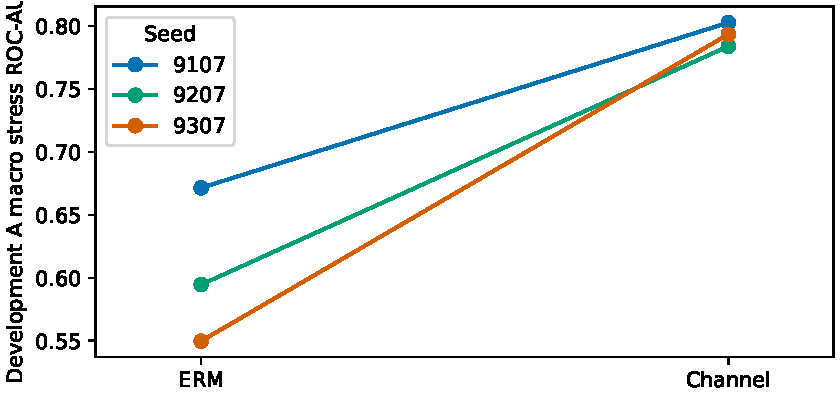
\includegraphics[width=.89\textwidth]{aggregate_v5.pdf}
\caption{Development macro stress ROC-AUC for the three initialization blocks. Lines connect the two arms within a seed.}\label{fig:aggregate}
\end{figure*}

The locked evaluation completed 17,408 predictions for the original four selected models. Table~\ref{tab:heldout-endpoints} reports aggregate results and Table~\ref{tab:heldout-conditions} separates the conditions. Macro stressed ROC-AUC increased in both seed blocks, from 0.8308 to 0.8875 in 9107 and from 0.7498 to 0.8948 in 9207. The corresponding paired speaker-cluster intervals for channel minus ERM were [0.0296, 0.0842] and [0.1158, 0.1752]. These positive differences were smaller than the development A contrasts. Figure~\ref{fig:heldout-contrasts} compares the predefined endpoints across partitions. Figure~\ref{fig:heldout-roc} shows the score-level ranking under each held-out condition.

Stressed FAKE misses fell from 1,370 to 587 in 9107 and from 815 to 453 in 9207, each out of 2,496 views from 832 FAKE sources. The rate differences were \ensuremath{-}31.37 points [\ensuremath{-}33.41, \ensuremath{-}29.36] and \ensuremath{-}14.50 points [\ensuremath{-}17.38, \ensuremath{-}11.67]. Stressed REAL false alarms increased by one in 9107, from 80/768 to 81/768 (+0.13 points), and fell from 322/768 to 136/768 in 9207. The 768 views in each comparison came from 256 REAL sources. The paired intervals were [\ensuremath{-}3.23, +3.76] and [\ensuremath{-}29.07, \ensuremath{-}19.03] percentage points. All endpoint and attack intervals used 10,000 valid draws.

\begin{table*}[t]
\centering
\small
\caption{Fixed-epoch training-size sensitivity for seed 9207 on the same development sources. Column headings give the training size. A has 112 sources per class and B has 144 REAL sources. Pooled stress counts use three views per source at threshold 0.5. Each attack row uses 18 sources.}\label{tab:size-sensitivity}
\begin{tabular}{@{}lrrrr@{}}
\toprule
Development endpoint & ERM 640 & Channel 640 & ERM 1,280 & Channel 1,280 \\
\colrule
A clean ROC-AUC & 0.9851 & 0.9809 & 0.9900 & 0.9860 \\
A macro stress ROC-AUC & 0.5946 & 0.7839 & 0.7062 & 0.8143 \\
A clean REAL false alarms & 4/112 & 4/112 & 1/112 & 3/112 \\
A clean FAKE misses & 9/112 & 9/112 & 3/112 & 8/112 \\
A stress REAL false alarms & 167/336 & 70/336 & 5/336 & 161/336 \\
A stress FAKE misses & 143/336 & 134/336 & 248/336 & 64/336 \\
B clean REAL false alarms & 26/144 & 20/144 & 18/144 & 22/144 \\
A05 stressed FAKE misses & 38/54 & 47/54 & 50/54 & 36/54 \\
A06 stressed FAKE misses & 16/54 & 31/54 & 50/54 & 11/54 \\
\botrule
\end{tabular}
\end{table*}


\begin{figure*}[t]
\centering
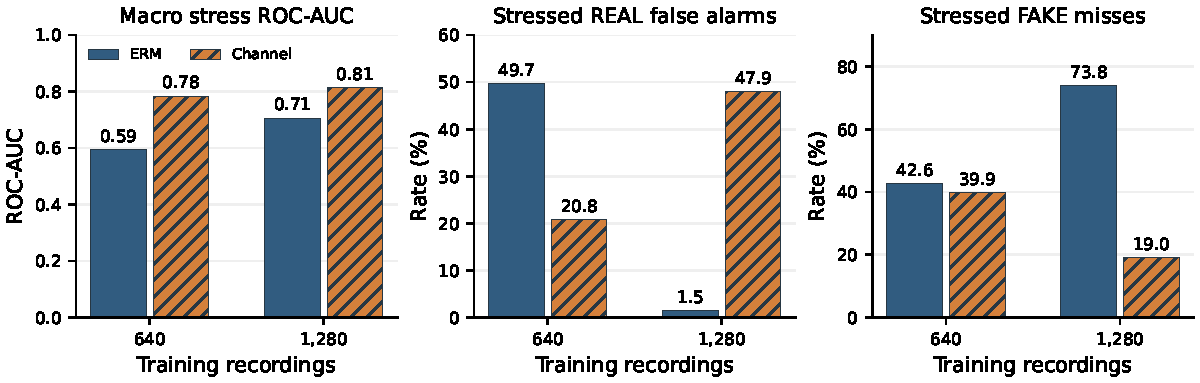
\includegraphics[width=.97\textwidth]{size_sensitivity_v7.pdf}
\caption{Seed-9207 development A results on the same recordings at both training sizes. Macro stress ROC-AUC averages three condition-level AUCs. Each pooled error rate uses 336 views from 112 sources of its class at threshold 0.5. Bars show observed values. Table~\ref{tab:size-sensitivity} gives counts and the text reports the paired intervals.}\label{fig:size-sensitivity}
\end{figure*}

\subsection{Class-Asymmetric Errors and Operating-Point Trade-offs}

With 1,280 samples, Channel improves stressed FAKE misses from 248 to 64 out of 336 (\ensuremath{-}54.76 points) and increases stressed REAL false alarms from 5 to 161 out of 336 (+46.43 points). With 640 samples, the respective contrast for REAL false alarms is \ensuremath{-}28.87 points, leading to a size contrast of +75.30 points (pointwise 95\% speaker interval [62.50, 87.80]). Figure~\ref{fig:size-sensitivity} illustrates that better ranking is accompanied by switching the class of errors at the threshold 0.5.

The selected 1,280 Channel checkpoint violates both registered +2-point clean-risk guards. Development A clean FAKE misses rose from 3/112 to 8/112 (+4.46 points) and B clean REAL false alarms rose from 18/144 to 22/144 (+2.78 points). Pointwise 95\% speaker intervals were [1.79, 6.25] and [\ensuremath{-}4.86, 11.81] percentage points. The B interval includes zero. The guards use the observed differences for the pair selected by clean BCE, so both exceed the tolerance.

Table~\ref{tab:conditions} breaks down the parts of the macro stress outcome. The table and ROC figure detail the first two seeds. The channel arm also increases AUC under all registered stress conditions in 9307. Figure~\ref{fig:roc} depicts the complete ROC curves associated with these AUCs. Fixed-threshold changes remain heterogeneous. Under Noise5, FAKE misses fall from 99 to 64 in 9107 and from 77 to 56 in 9207. The corresponding REAL false-alarm counts rise from 1 to 8 in 9107 and fall from 22 to 13 in 9207.

\begin{table*}[t]
\caption{Selected-model results on the locked held-out subset. Stress error counts pool three views per source. Macro stress ROC-AUC averages the three condition-specific AUCs.}\label{tab:heldout-endpoints}
\centering
\small
\begin{tabular}{@{}lrrrr@{}}
\toprule
Endpoint & 9107 ERM & 9107 Channel & 9207 ERM & 9207 Channel \\
\colrule
Macro stress ROC-AUC & 0.8308 & 0.8875 & 0.7498 & 0.8948 \\
Stress FAKE miss & 1370/2496 & 587/2496 & 815/2496 & 453/2496 \\
Stress REAL false alarm & 80/768 & 81/768 & 322/768 & 136/768 \\
Clean REAL false alarm & 25/256 & 19/256 & 22/256 & 16/256 \\
Clean FAKE miss & 125/832 & 129/832 & 127/832 & 147/832 \\
\botrule
\end{tabular}
\end{table*}


\begin{table*}[t]
\caption{Condition-specific held-out performance. Each cell gives ROC-AUC / REAL false alarms / FAKE misses. There are 256 REAL and 832 FAKE recordings per condition.}\label{tab:heldout-conditions}
\centering
\small
\begin{tabular}{@{}lrrrr@{}}
\toprule
Condition & 9107 ERM & 9107 Channel & 9207 ERM & 9207 Channel \\
\colrule
Clean & 0.9534 / 25 / 125 & 0.9436 / 19 / 129 & 0.9507 / 22 / 127 & 0.9410 / 16 / 147 \\
Noise5 & 0.8053 / 0 / 701 & 0.8655 / 12 / 259 & 0.6815 / 28 / 492 & 0.8765 / 25 / 193 \\
Noise to Opus & 0.8447 / 76 / 143 & 0.8991 / 53 / 143 & 0.8196 / 226 / 38 & 0.9044 / 89 / 93 \\
Opus to noise & 0.8424 / 4 / 526 & 0.8979 / 16 / 185 & 0.7483 / 68 / 285 & 0.9034 / 22 / 167 \\
\botrule
\end{tabular}
\end{table*}


The larger 9207 REAL benefit under the two compositions is visible in the per-condition counts. Noise-to-Opus false alarms fall from 104 to 44, while its FAKE misses increase from 13 to 26. By way of contrast, REAL false alarms go from 41 down to 13, while FAKE misses go from 53 down to 52. Both counts have denominator 112. The starting point with the high number of REAL false alarms for the condition of Noise-to-Opus allows a sizable decrease in this operating point. It would not be accurate to refer to the decrease itself as an advantage across classes.

For the stress results, gain controls and Opus64 for the two development seeds give some perspective. For quarter gain, the channel arm has fewer false alarms and higher AUC in both blocks. For standalone Opus64, the channel arm has fewer false alarms but higher FAKE misses in both blocks. The control of 64 kb/s uses a different rate from the compositions of 24 kb/s. It is listed as a separate condition, and any comparison against the chains would alter the codec and noise conditions as well. The 24 kb/s control is the correct one for standalone comparison against 9107 and 9207.

In 9307, stress FAKE misses fall from 266 to 119 of 336 while REAL false alarms rise from 44 to 61 of 336. This contrasts with fewer stressed REAL false alarms in 9107 and 9207. The 9307 stress miss contrast is \ensuremath{-}43.75 percentage points (95\% speaker interval [\ensuremath{-}47.92, \ensuremath{-}39.58]). The contrast for its stress REAL false alarm is +5.06 points (interval [\ensuremath{-}1.79, +10.42]). B clean false alarms increase from 21 to 30 out of 144, which is a change of +6.25 points (95\% speaker interval [\ensuremath{-}1.39, +15.28]). The difference is greater than the registered +2-point guard for the selected CLEAN\_BCE pair. The interval represents speaker resampling in the pair and does not affect the observed guard choice.

In 9207, decreases in other attack instances balance 24 extra A05 and A06 missed instances under stress conditions. The A05 and A06 attacks add six extra missed instances in 9107. The differences include transformed views. Table~\ref{tab:attackconditions} gives the number of A05 and A06 attacks that get an additional correct or missed decision in at least one stress condition. Figure~\ref{fig:transitions} provides the paired analysis for both classes under A.

\begin{figure*}[t]
\centering
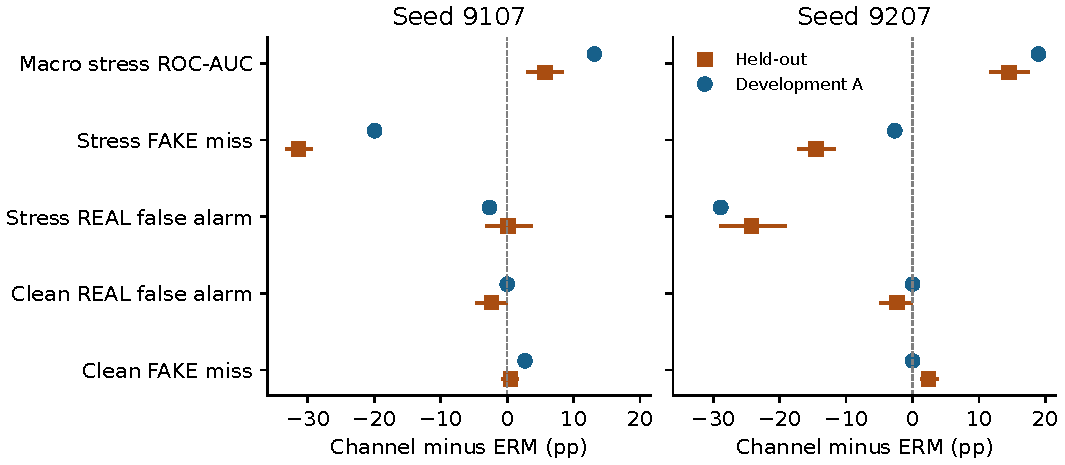
\includegraphics[width=.94\textwidth]{heldout_contrasts.pdf}
\caption{Channel-minus-ERM contrasts on development A and the locked held-out subset, separately by seed. Held-out segments show 95\% paired speaker-cluster percentile intervals. AUC differences are multiplied by 100. Positive differences indicate better AUC or higher error rates. Cohorts and attack populations differ across partitions.}\label{fig:heldout-contrasts}
\end{figure*}

Clean REAL false alarms fell from 25 to 19 in 9107 and from 22 to 16 in 9207, out of 256 sources per arm. Clean FAKE misses increased from 125 to 129 and from 127 to 147 out of 832, while clean ROC-AUC declined from 0.9534 to 0.9436 and from 0.9507 to 0.9410. The 9207 clean FAKE miss increase was 2.40 percentage points [1.15, 3.86]. Development B showed opposite false-alarm directions between the two seeds. The cohorts differ in speaker and source support.

The sums for stress reflect the existence of the operating point shift. For Noise5, the misses of FAKE dropped from 701 to 259 and from 492 to 193 out of 832. With respect to Opus and then Noise10, the misses of FAKE dropped from 526 to 185 and from 285 to 167. In case of the reverse sequence, Noise10 followed by Opus, the misses of FAKE remained constant at 143 in 9107 and increased from 38 to 93 in 9207, while the number of REAL false alarms decreased from 226 to 89 out of 256 and AUC increased from 0.8196 to 0.9044.

Post hoc analysis shows that at the threshold of 0.5 the operating point has shifted. When Noise10 and then Opus were applied in 9207, the two algorithms agreed on 85 real false alarms, channel corrected 141 and made four. In case of FAKE, they agreed on 20 misses, channel corrected 18 and introduced 73. In 9107, when the two algorithms were subjected to Noise10 and then Opus, the sum of 143 FAKE misses included 93 shared misses, 50 corrected and 50 introduced. The numbers reflect decision-making on the same sources.

In Fig.~\ref{fig:v4-operating}, the retro-grid ensures that the registered threshold remains at 0.5. On held-out 9207 under Noise10 followed by Opus24, channel augmentation gives fewer false alarms and more misses at every sampled threshold from 0.20 through 0.80. The miss direction reverses at 0.10 and 0.90. For Noise5 and the opposite order, FAKE misses decrease at all 11 sampled thresholds in both seeds, with condition- and seed-dependent REAL errors. FAKE misses cleaned in 9207 rise for all thresholds sampled. These comparisons describe the measured score grid and provide no threshold-selection rule.

Score distributions also change locally around the registered boundary. Under Noise10 followed by Opus24 in 9207, 7 versus 30 of 256 REAL scores and 5 versus 18 of 832 FAKE scores lie within 0.025 of 0.5 for ERM and channel, respectively. The supplement gives the confusion matrices for every arm and condition, empirical curve coordinates and the 0.025 and 0.05 score windows. Development B supplies only REAL scores. Its FNR, ROC-AUC and EER are undefined.

\begin{figure*}[t]
\centering
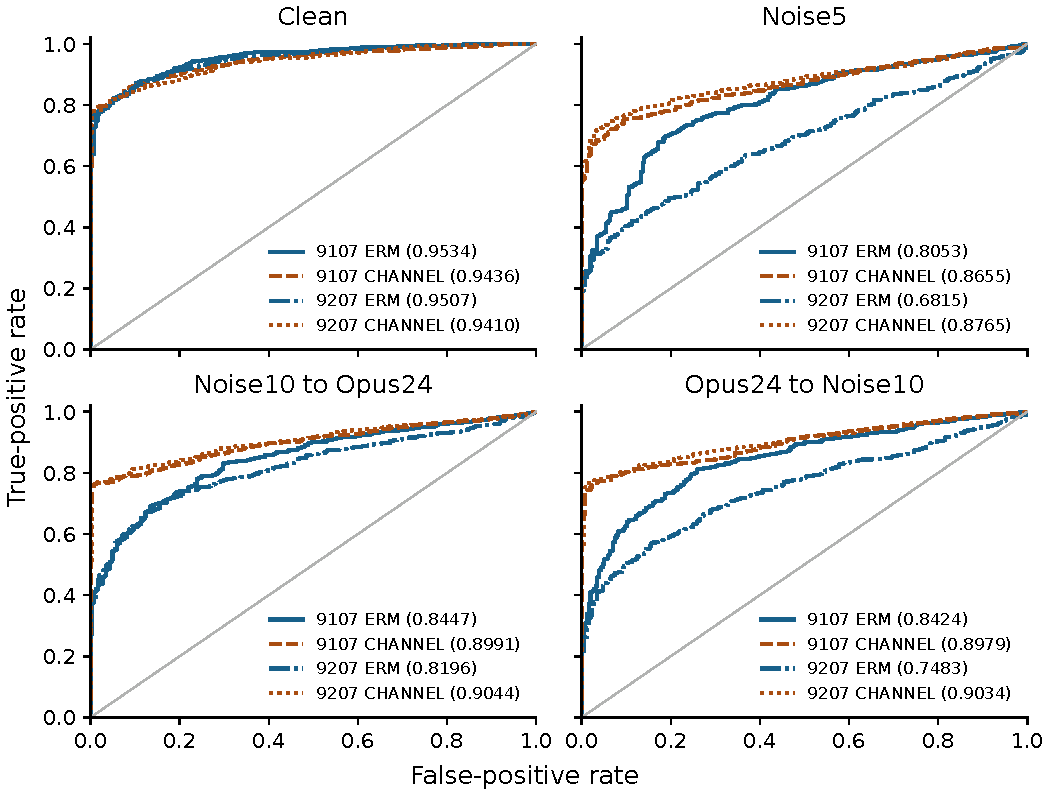
\includegraphics[width=.86\textwidth]{heldout_roc.pdf}
\caption{Empirical held-out ROC curves for four selected models. Each panel contains 256 REAL and 832 FAKE recordings, evaluated under the named condition. Legends give seed, method, and AUC. The same sources recur across conditions.}\label{fig:heldout-roc}
\end{figure*}

\subsection{Attack-Specific Robustness and Failure Modes}

For seed 9207, the A05 contrast changes from 38/54 versus 47/54 at 640 to 50/54 versus 36/54 at 1,280 (ERM versus Channel). A06 changes from 16/54 versus 31/54 to 50/54 versus 11/54. Each denominator represents three correlated stress views from 18 sources. Both training size and update budget changed. Seed 9307 compares initializations at 640. Table~\ref{tab:attack} and Fig.~\ref{fig:attack} show both sign reversals. Channel increases A05 and A06 stress misses in the first two pairs and decreases them in 9307. The latter changes are \ensuremath{-}6/54 and \ensuremath{-}17/54, respectively. The pointwise 9307 speaker intervals are [\ensuremath{-}16.67, \ensuremath{-}5.26] and [\ensuremath{-}43.86, \ensuremath{-}17.54] percentage points, respectively. The 9107 intervals include zero. These within-seed intervals do not establish a stable attack effect across initializations.

Table~\ref{tab:attackconditions} details the first two seeds. In 9307, all six A05 recoveries occur in the noise-before-Opus condition. For A06, 18 recoveries and one new miss occur across the three stress views. Net recoveries span five A05 speakers and six A06 speakers. The A06 ERM burden is 16 of 54 in 9207 and 45 of 54 in 9307. Differences in baseline burden and FAKE score crossings describe where the reversal occurs. They leave the underlying model or generator mechanism unresolved.

\begin{figure*}[t]
\centering
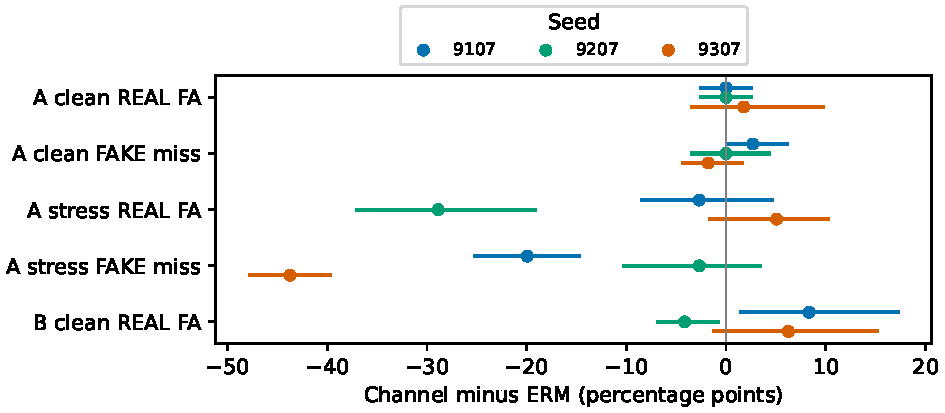
\includegraphics[width=.91\textwidth]{classwise_errors_v5.pdf}
\caption{Channel-minus-ERM fixed-threshold error rates by development stratum, class, and seed. Segments show within-seed paired speaker-cluster percentile intervals. REAL errors are false alarms and FAKE errors are misses. Clean A has 112 recordings per class, stress A has 336 views from 112 recordings per class, and clean B has 144 REAL recordings.}\label{fig:classwise}
\end{figure*}

\begin{table*}[t]
\centering
\small
\caption{Development A05/A06 stress FAKE misses over the three stress views. Each row represents 18 distinct sources and 54 transformed views.}\label{tab:attack}
\begin{tabular}{@{}lrrr@{}}
\toprule
Seed and attack & ERM & Channel & $\Delta$ misses \\
\colrule
9107 A05 & 48/54 & 50/54 & +2 \\
9107 A06 & 41/54 & 45/54 & +4 \\
9207 A05 & 38/54 & 47/54 & +9 \\
9207 A06 & 16/54 & 31/54 & +15 \\
9307 A05 & 49/54 & 43/54 & -6 \\
9307 A06 & 45/54 & 28/54 & -17 \\
\botrule
\end{tabular}
\end{table*}


Figure~\ref{fig:speakers} shows that two B speakers contribute 10 of the 12 net additional false alarms in 9107. For 9207, reductions occur across several speakers. B contains only REAL recordings, and the counts are interpreted as false alarms with no B ROC-AUC or EER.

Figure~\ref{fig:heldout-attacks} shows the condition-specific FAKE miss contrasts. Pooled stressed misses fell on A07--A16 and rose on A17--A19 in both blocks. A17, A18 and A19 added 10, 11 and 4 misses in 9107 and 43, 43 and 56 in 9207, each out of 192 views from 64 sources per attack. The pointwise 9107 intervals include zero. The 9207 intervals exclude zero: [15.90, 29.03], [14.12, 30.81] and [20.63, 37.70] percentage points. The development A05/A06 results concern a separate attack set.

In the post-hoc grouping, A07--A16 account for 808 and 504 fewer stressed misses in 9107 and 9207, partly offset by 25 and 142 additional misses on A17--A19. For A17--A19, Noise-to-Opus added 39 misses in 9107. All three stress conditions added misses in 9207. On A19, 43/64 sources acquired a miss in at least one stress condition and 18/64 in multiple conditions. These exploratory groupings were identified after reviewing held-out results. The pointwise intervals have no multiplicity adjustment.

\begin{figure*}[t]
\centering
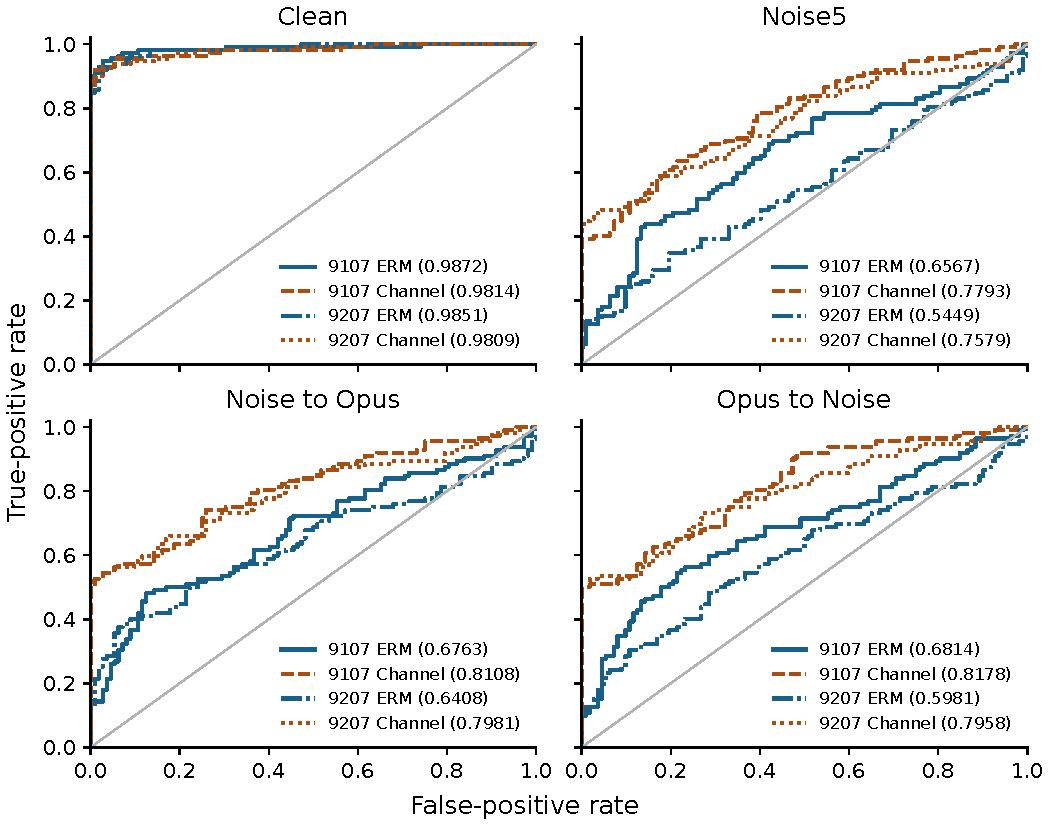
\includegraphics[width=.88\textwidth]{development_roc.pdf}
\caption{Empirical ROC curves from the four selected models in the first two seeds on development A. Each panel ranks the same 112 REAL and 112 FAKE recordings under one condition. Legends give the seed, method, and recomputed AUC. The diagonal denotes chance ranking.}\label{fig:roc}
\end{figure*}

\subsection{Transformation-Order Effects}

For the same 112 A REAL recordings at seed 9207, the Channel-minus-ERM contrast in the signed order error gap (Noise-to-Opus minus Opus-to-Noise) changes from \ensuremath{-}28.57 points at 640 to +26.79 points at 1,280. The size contrast is +55.36 points (pointwise 95\% speaker interval [32.12, 79.46]). The change in the corresponding signed FAKE-score difference is \ensuremath{-}0.2099 to +0.0764. These paired contrasts measure detector response to the order of processing. See the supplement for the counts exclusive and inclusive to each arm and class. In the first two development blocks, out of 112 A REAL sources, the Noise-to-Opus-only false-alarm counts change from 43 to 19 in 9107 and 63 to 31 in 9207. The opposite order has no exclusive REAL false alarms in A. Among 112 A FAKE sources, Opus-to-Noise alone causes 48 versus 17 misses in 9107 and 40 versus 26 in 9207. The Noise-to-Opus-only FAKE counts are 1 versus 0 and 0 versus 0. In the 9307 pair, there is also the same order asymmetry classwise. Noise-to-Opus-only REAL errors have shifted from 37 to 44, while Opus-to-Noise-only FAKE errors have shifted from 41 to 33, both in a sample of 112. The signed FAKE score gap decreases from 0.2375 to 0.0538 in the median. Figure~\ref{fig:order} represents paired score differences before the thresholding point.

9107 retrospective diagnostics produce 1,472 predicted values for Noise10 and Opus24 separately. Matched waveforms help recover not only registered sequences but also selected anchor values that were replayed without drifting. A leave-one-speaker-out nuisance regression yields directional class-discrimination AUCs of 0.538 for ERM and 0.432 for channel on the signed order score. This measures a residual score contrast on the development cohort. The same standalone components were evaluated for seed 9207 on all 368 development sources, adding 1,472 predictions. All 18 clean and ordered score anchors matched their sealed values exactly. On development A, standalone Noise10 FAKE misses decreased from 82 to 54 in 9107 and changed from 47 to 48 in 9207, out of 112 per arm. Under standalone Opus24, 9207 REAL false alarms decreased from 19 to five and FAKE misses increased from two to ten. The 9107 nuisance regression remains a single-seed analysis. These component results constrain interpretation of the compositions and do not identify a forensic mechanism.

\begin{figure*}[t]
\centering
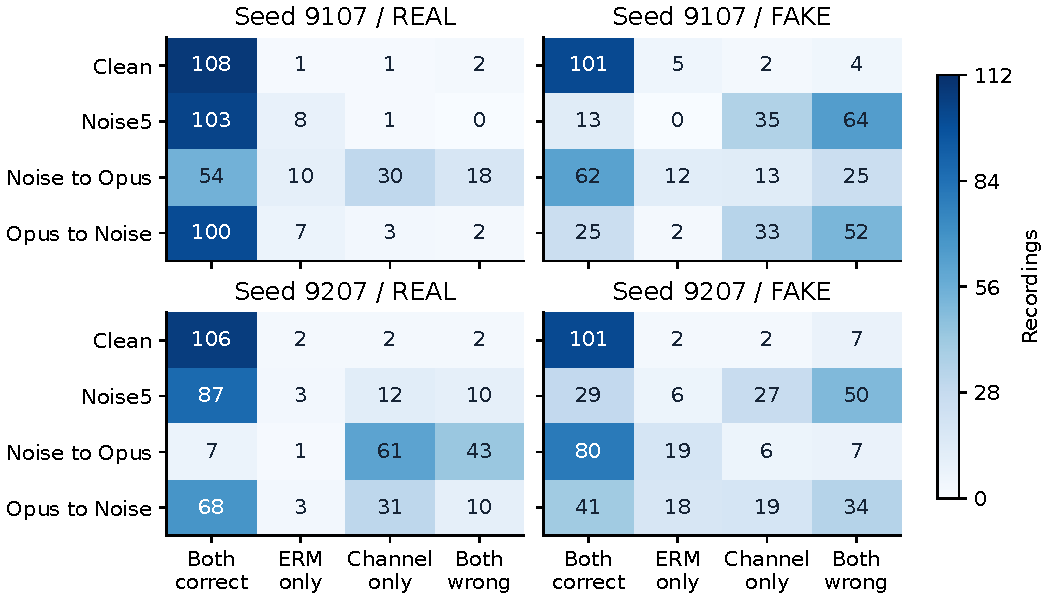
\includegraphics[width=.96\textwidth]{source_transitions.pdf}
\caption{Within-source correctness for the first two seeds at threshold 0.5 on development A. Each row contains 112 recordings of the indicated class. The same recordings contribute to each condition row. The two middle columns identify sources correctly classified by only one method.}\label{fig:transitions}
\end{figure*}

\begin{table*}[t]
\caption{A05 and A06 source-level diagnostics. Each condition has 18 sources. Error cells are ERM / channel. Harm and recovery can overlap across views.}\label{tab:attackconditions}
\centering
\small
\begin{tabular}{@{}lrrrrrr@{}}
\toprule
Seed / attack & Clean & Noise5 & Noise to codec & Codec to noise & All stress & Harmed / rec. \\
\colrule
9107 / A05 & 0 / 0 & 17 / 17 & 14 / 16 & 17 / 17 & 14 / 16 & 3 / 1 \\
9107 / A06 & 3 / 6 & 18 / 16 & 7 / 12 & 16 / 17 & 6 / 12 & 7 / 2 \\
9207 / A05 & 0 / 0 & 17 / 17 & 7 / 13 & 14 / 17 & 7 / 13 & 8 / 0 \\
9207 / A06 & 5 / 7 & 9 / 12 & 0 / 5 & 7 / 14 & 0 / 5 & 10 / 0 \\
\botrule
\end{tabular}
\end{table*}


Source-linked order asymmetry persisted. In 9107, REAL sources wrong only under noise-to-Opus numbered 72 for ERM and 37 for channel, with zero exclusive errors in the reverse direction. In 9207 the corresponding counts were 158 and 68, while exclusive reverse-order errors numbered zero and one. Among FAKE sources, reverse-order-only misses numbered 384 and 43 in 9107 and 247 and 74 in 9207. The opposite exclusive FAKE miss counts were one and one in 9107, and zero and zero in 9207. Each model uses the same 256 REAL and 832 FAKE sources in the order comparison.

\begin{figure*}[t]
\centering
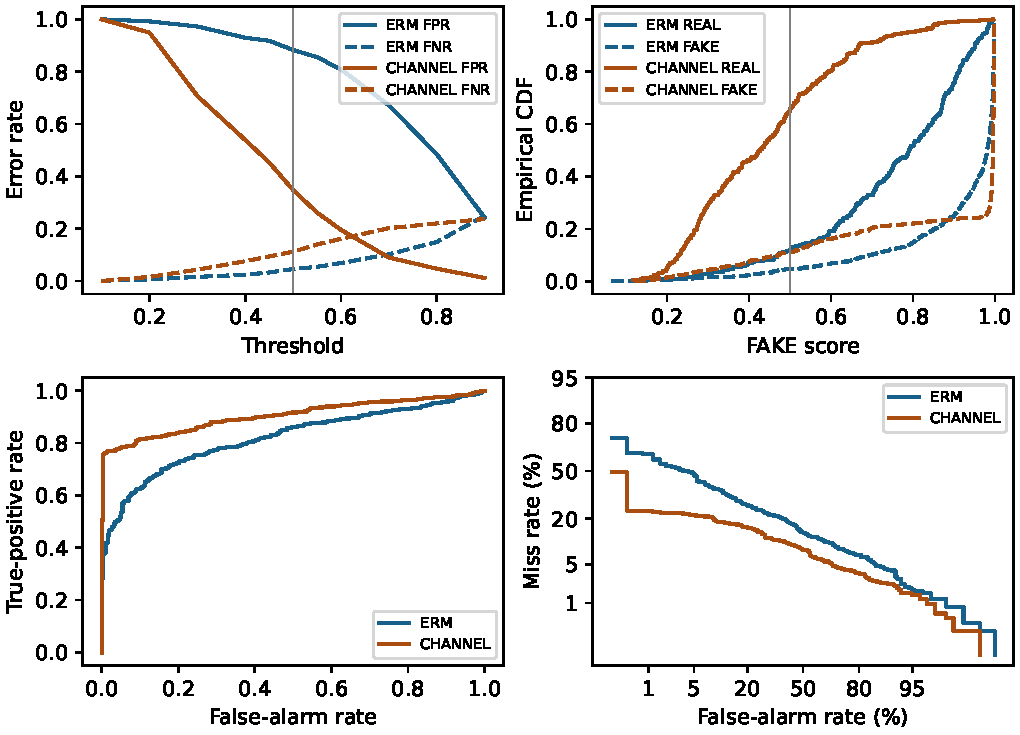
\includegraphics[width=.95\textwidth]{operating_points_v4.pdf}
\caption{Held-out seed 9207 under Noise10 followed by Opus24. Top left shows exploratory FPR and FNR at 11 thresholds. Top right shows class-specific empirical CDFs. Bottom panels show empirical ROC and DET. DET axes use a normal quantile transform and clip endpoint rates at half an event per class. The vertical lines identify the registered threshold of 0.5. Each arm has 256 REAL and 832 FAKE sources.}\label{fig:v4-operating}
\end{figure*}

The score contrasts shown in Fig.~\ref{fig:heldout-order} were also directional, with reduced median FAKE scores following channel adaptation. The median score contrasts in FAKE became 0.3454 and 0.0063 in 9107, 0.2419 and 0.0076 in 9207. However, small score contrasts cannot automatically be assumed to reflect a superior decision rule, in view of the fact that attack-specific misses occurred. Speaker-related scores exhibit the same order error pattern distribution. In the case of ERM 9107, the reverse-minus-forward FAKE error contrast was 16 out of 21 FAKE recordings for speaker LA\_0045 and 13 out of 21 for speaker LA\_0046.

\subsection{Robustness, Stability and Generalization}

The direction of the development stress ranking gain and FAKE miss reduction is consistent across all three pairs. The magnitude of the gain, as well as the direction of false-alarm results, varies according to the selected pair. Common development data allow for a comparison of initializations using the protocol described above, in which case speaker uncertainty is computed in each pair separately.

The fixed epoch size experiment includes a development-only comparison for seed 9207. The three initializations correspond to 640 recordings. The held-out evaluation evaluates the original 640 recording model corresponding to seeds 9107 and 9207 using additional ASVspoof 2019 LA speakers. Cross-corpus robustness remains untested.

\begin{figure*}[t]
\centering
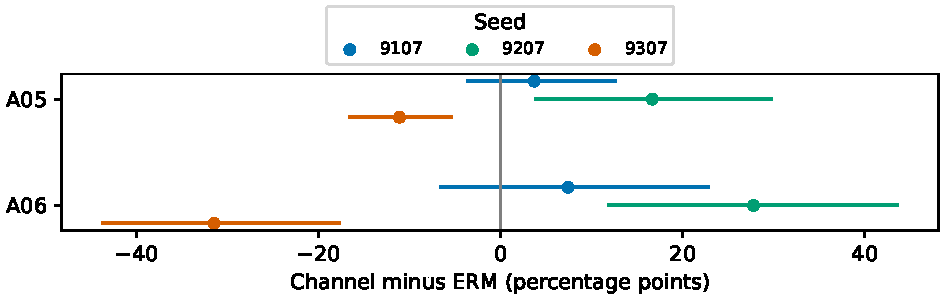
\includegraphics[width=.79\textwidth]{attack_changes_v5.pdf}
\caption{Development A05/A06 stressed FAKE miss changes by seed. Positive values indicate more misses. Intervals resample speakers within a seed. Each attack contributes 54 views from 18 recordings.}\label{fig:attack}
\end{figure*}

\begin{figure*}[t]
\centering
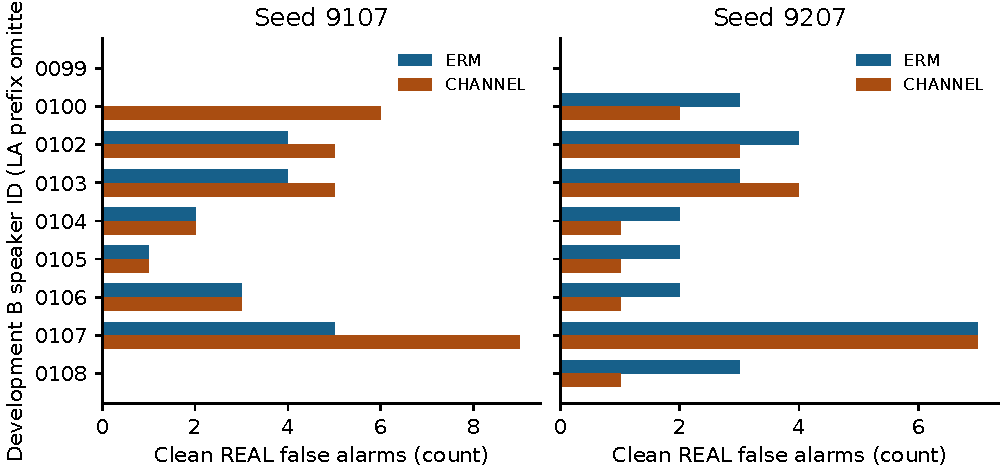
\includegraphics[width=.89\textwidth]{speaker_counts.pdf}
\caption{Clean REAL false alarms by speaker on development B for the first two seeds. Each of nine speakers contributes 16 recordings, for 144 recordings per arm and seed.}\label{fig:speakers}
\end{figure*}

\subsection{Practical Implications and Limitations}

In 9307 the recorded optimizer durations were 39.9 minutes for ERM and 78.9 minutes for channel. At 1,280, the seed-9207 optimizer durations were 78.6 and 160.3 minutes, respectively, with validation taking 37.6 and 37.9 minutes. These are local CPU workload measurements. The architecture and parameter count are shared across training sizes.

A bounded inference benchmark used the clean inputs of the first 12 registered development sources, repeated three times after anchor replay, at batch size one on a single CPU thread. Input duration was capped at 3 s. Median preprocessing time was 10.9 ms (interquartile range 10.3--11.2 ms), forward time 91.3 ms (90.5-93.5 ms), and end-to-end time 102.1 ms (101.1-104.2 ms). The timed preprocessing includes decoding, resampling and the P0 input transform on clean input. The separate headroom and channel-transform stages are outside the timed path. The two 9207 exports each contain 1,308,401 parameters, of which 369,281 are updated during warm-up and 646,481 during partial fine-tuning. The exported stage has 661,920 nontrainable parameters. Each export occupies 5,916,699 bytes. Loading time in one process was 3.35 and 2.81 s, where the second loading came after the first loading. The maximum process working set during the timing process was about 475 MiB. The development convenience sample supports an architectural and local runtime description. Mobile, streaming and concurrent performance remain unmeasured.

\begin{figure*}[t]
\centering
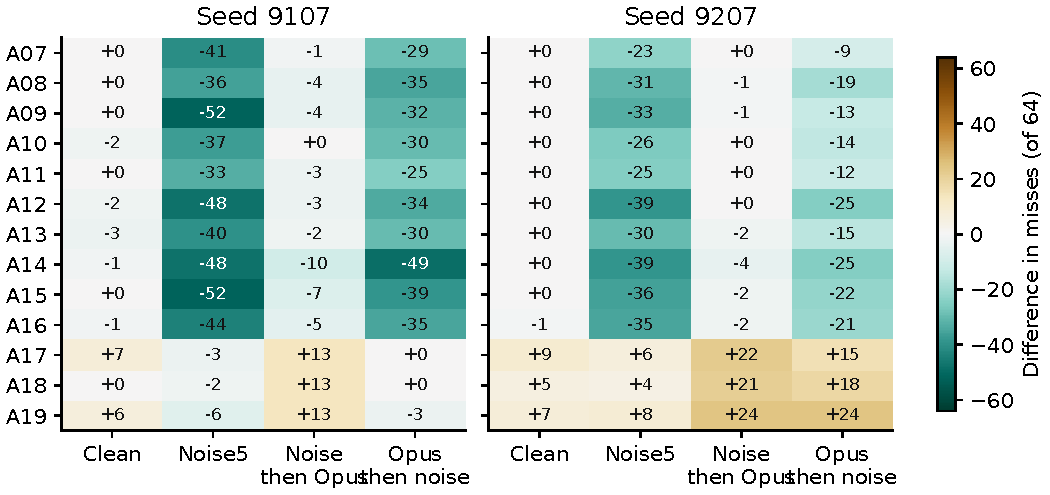
\includegraphics[width=.92\textwidth]{heldout_attacks.pdf}
\caption{Held-out channel-minus-ERM FAKE miss counts by attack, condition and seed. Each cell compares the same 64 sources. Positive counts indicate deterioration and negative counts indicate fewer misses. The full numerical supplement retains both arm counts and stressed attack intervals.}\label{fig:heldout-attacks}
\end{figure*}

The error curves illustrate why a new operating point requires independent validation with costs and traffic prevalence appropriate to the deployment. The ordered chains make it more imperative to validate the position where noise is added vis-a-vis codec operations.

\section{Discussion}\label{sec:discussion}
Aggregate stressed ranking improves in both observed blocks, with a mean difference of approximately 0.1602 ROC-AUC units. A cleaner separation of many stressed sources can raise the average even if particular attack groups shift below the chosen threshold. The measured changes in attacks A01, A03 and A04 and the worsening on A05 and A06 show why aggregate ranking is insufficient for selecting an operating point. The latter two attacks are represented in training. Their deterioration reflects a within-benchmark robustness gap under the tested intervention.

The error effect depends on initialization. The A stressed FAKE miss reduction is larger for 9107, and the 9207 cluster interval includes zero. Clean B false alarms move in opposite directions, with the 9107 increase concentrated in two speakers. Changing the score distribution relative to 0.5 could contribute to these changes, even if discrimination improves. The results describe decisions under the registered threshold and do not evaluate threshold recalibration.

For many REAL sources, Noise-to-Opus is the only erroneous order. For FAKE sources, the reverse chain is often the only erroneous order. An upward shift in FAKE scores under one order can produce both patterns. The retrospective matched-component diagnostic for 9107 finds that nuisance adjustment does not establish an independent forensic target. Nonlinear codec response, preprocessing, and detector sensitivity may all contribute. Reproducing the direction of decision asymmetry in 9207 does not independently reproduce the nuisance analysis.

In practical evaluation, reporting both threshold-specific risks and ranking separates several failure modes that may have different costs. Speaker concentration also affects how a review workload might change, although no field workload or utility was measured. Conventional Opus order reversal, class-wise counts and a matched training intervention provide a focused complement to broader robustness benchmarks and codec-adaptation methods.

\subsection{Aggregate improvement and its distribution}
The matched comparison makes training-view policy the controlled factor, but does not isolate a single cause inside the fitted network. The channel model can learn features that distinguish more stress-processed pairs, move score distributions relative to the fixed decision boundary, or do both. Clean BCE selection may choose a different epoch in each arm because the fitted score distributions are different. The observed contrast therefore includes the interaction of augmentation with the same selection rule. It cannot determine which intermediate representation would be responsible, or how an alternate selection rule would change outcomes.

The adverse results for A05 and A06 matter in two distinct ways. First, these groups already contribute repeated stress errors before augmentation. Their denominators are small, so an individual source can affect several condition counts. Second, the registered model comparisons show additional errors distributed across several sources, especially in the 9207 block. The per-condition breakdown distinguishes an attack already difficult under Noise5 from additional failures concentrated in the ordered compositions. This supports a localization claim about the tested inputs. It does not show which characteristics of their synthesis pipelines caused the effect.

REAL false alarms can shift if a score displacement moves bona fide examples near 0.5 across the threshold. In B the two blocks move in opposite directions, and part of the 9107 increase concentrates in a small number of speakers. Bona fide cross-testing work makes the broader case for assessing bona fide diversity \cite{kwok}. Our speaker analysis addresses a narrower issue inside one fixed cohort. A different bona fide corpus, language, noise mixture or deployment prior could change both the baseline rates and the direction of the intervention effect.

\subsection{Signal-chain and engineering implications}
Published communication benchmarks such as ADD-C vary codec and packet-loss conditions \cite{addc}. Their breadth is useful for establishing stress coverage. The same-source order contrast here trades breadth for experimental control. It compares two explicitly defined pipelines at fixed settings and records exactly which order makes a particular decision fail. The association can motivate a follow-up test with actual transmission and varied gain controls. It cannot stand in for that test because the present experiment omits network loss and device processing.

Where a review decision is threshold based, a deployment report should specify the order and settings of the signal-processing chain and give error counts by class. A rank statistic can summarize detector ordering, and an error transition table can show whether a system has shifted errors to a different group. The latter is valuable even if total counts tie. For example, two methods can flag the same number of bona fide sources but require review of different recordings. No application-specific cost or calibration was measured, so a cost-optimal operating rule remains a separate problem.

The present controlled intervention uses ordinary BCE and one view per source. Its scientific contribution is the error accounting and the evidence that the observed rank benefit coexists with subgroup deterioration. Extending the claim would require a locked independent partition, then genuinely new corpora or models to measure broader transport. Confirmation of a forensic mechanism would additionally require a cue definition and a measurement that can vary independently of the detector output.

\subsection{From a validation metric to a validation workflow}
For an engineer deciding whether to adopt augmentation, the condition table distinguishes several cases. An AUC increase with reductions in both error types shows improvement at both levels measured. An AUC increase with fewer false alarms and more misses indicates that a rank gain and an operating-point trade-off coexist. A near-tie in counts can still conceal a change in the individual sources that require attention. The present results exhibit these behaviors under different conditions. A validation workflow benefits from retaining source identity through the paired analysis.

Nominal condition names can also obscure the processing intervention. A label that names noise and Opus omits whether the noise is present during coding. The operator descriptions here fix that detail and define how the noise realization is shared. This isolates sensitivity to the specified order without assuming either chain represents all communication paths. It also motivates reporting codec rates alongside order. Opus64 has different settings and support from the 24~kb/s compositions, and their contrast cannot isolate bitrate. The present evidence pertains to a classifier after specified transformations. A claim about forensic cue retention would require a separate measurement that varies independently of classifier output.

\subsection{Evidence needed to extend the claim}
The conference reviewers raised related questions about broader robustness and repeatability. The journal makes progress by separating training initialization from test-source resampling, documenting how the operating rule interacts with class-specific effects, and retaining source links through the analysis. These changes address inference and diagnosis within the registered scope. They leave broader shifts unresolved. The appropriate next empirical test is whether the same fixed models preserve the observed directional trade-offs on the locked within-release cohort. A benchmark result there would still leave the external-corpus, physical channel and multi-architecture questions open.

If the held-out ranking gain weakens or the error trade-off changes, both outcomes belong in the main results. In particular, the observed A05 and A06 development errors cannot be projected directly onto A07 through A19. The official corpus documentation relates some attack algorithms across partitions, and the five-column metadata does not identify full generator lineage. The scientific conclusion should therefore be phrased in terms of the designated partitions and conditions. Claims of genuinely unseen generator robustness require an additional design with independently verified generator provenance.

\subsection{Reporting a locked follow-up}
The interpretation of a subsequent held-out comparison should distinguish transport of the aggregate direction from transport of each conditional error pattern. If both stress ranking differences remain positive, the result would extend the observed direction to the registered evaluation partition. The fixed-threshold errors would still require separate reporting by class and condition. A change in the FAKE miss direction would be informative even in the presence of a rank benefit. The development A05 and A06 observations should remain in the paper regardless of the held-out outcome because the attack sets and source populations differ.

The primary held-out set deliberately allocates equal quotas to the registered FAKE attacks. This helps make support transparent and reduces the influence of an attack merely having more available archive records. It does not reproduce real-world spoof prevalence. Attack-stratified misses and class-conditional errors therefore remain more interpretable than an isolated accuracy figure. The same selection constraints and scores must apply to every model. Reporting the number of sources and views together will also prevent a complete set of predictions from being mistaken for an equal number of independent utterances.

The four frozen detectors provide two paired comparisons. A common pattern across the held-out models would add evidence about these fit blocks and this partition. It would leave random-initialization variability beyond the two observed seeds, language transport, and architecture transfer unresolved. Conversely, an adverse held-out contrast should be documented without changing the threshold or subset in response. Any future recalibration or modification of the augmentation bank would define a new intervention and require a new evaluation contract. This separation protects the difference between a planned test and an exploratory diagnosis after observing its results.

\section{Limitations and Threats to Validity}\label{sec:limits}
The 640-source cohort is a compute-bounded training design. It does not represent full-foundation training. A and B have limited speaker support, and attack groups have 18 or 19 sources. The bootstrap describes uncertainty under speaker resampling on these fitted models and this cohort. Related conditions within a source are dependent. Secondary subgroup diagnostics are descriptive and no multiplicity adjustment is implied.

The two initialization blocks share the same development data and checkpoint rule. The same partition supports checkpoint selection and the reported development analysis. The results are sensitive to the fixed decision threshold and selected checkpoint. In particular, guard failure applies to the selected checkpoint comparison. It does not imply that every epoch or threshold would fail.

Only one architecture was retrained in the matched design. Signal preprocessing, noise scaling, and codec response can change the score contrast independently of forensic cue retention. The current experiments provide no verified independent forensic target. The pending official evaluation is within the same corpus release, and some evaluation attacks reuse algorithms or frameworks. Cross-corpus, cross-architecture, and deployment robustness remain open.

\section{Conclusion}
The experiment supports an evaluation practice for lightweight speech countermeasures. Rank metrics describe the ordering of authentic and spoofed recordings, while fixed-threshold and paired transition counts identify which decisions change after a specified audio-processing chain. When those measurements are reported together, the augmentation benefit is more precisely defined. It extends to stressed ranking in both tested initialization blocks, while A05 and A06 deteriorate at the fixed threshold and the REAL-only false-alarm difference depends on the block.

The source-linked order analysis establishes that the two processing orders produce different detector responses under the tested settings. The available evidence leaves the underlying forensic mechanism unresolved. A locked within-release evaluation will test whether the empirical trade-offs transfer to the designated benchmark partition. Broader transfer would require additional corpora and models with explicitly defined operating conditions.


\section*{Reproducibility}

The experiment registries, per-source scores, checkpoint seals, and speaker-bootstrap outputs document eight development fits and the original four-model locked evaluation. The supplement identifies the four selected seed-9207 checkpoints used for the size contrast and provides the registered endpoints, pointwise speaker intervals, order transitions and execution costs. The analysis code reproduces the size contrast from the sealed development scores. It also records the three-seed 640 analysis and the retrospective threshold and standalone component diagnostics. Section~\ref{sec:setup} defines the evaluation populations.

The locked protocol \texttt{r08\_external\_v1} records the release, the selection seed and the hashes of the 512 recordings and six selected checkpoints. The selected-row SHA-256 is \texttt{51cd5643}\allowbreak \texttt{dbf6df7c}\allowbreak \texttt{6f6cfe2d}\allowbreak \texttt{3dfa8e8a}\allowbreak \texttt{d0371fa0}\allowbreak \texttt{d5d6d900}\allowbreak \texttt{687adeb5}\allowbreak \texttt{38ed3e38}. The registered run records P0, the 0.5 decision threshold, source-level scores and a verified seal for 3,072 predictions and two aggregate files. The metadata do not resolve original parent-source relationships.

\section*{Data Availability}
ASVspoof 2019 LA is third-party data distributed by the \href{https://doi.org/10.7488/ds/2555}{University of Edinburgh}. The pinned In-the-Wild release is distributed through the \href{https://huggingface.co/datasets/mueller91/In-The-Wild/tree/eee168f92c367f8c82ff2cf42b6f61e362fd6211}{dataset repository} \cite{wild}. Distributor terms permit local evaluation and reporting of aggregate results. The project retains raw external WAV files locally. Author-generated manifests and predictions are archived with the run, and their sharing is subject to the applicable dataset conditions.

\section*{Code Availability}
The project source and reproducibility scripts are available in the \href{https://github.com/datweb07/audio-deepfake-mobilenet-lstm}{project repository}. Reproduction also requires separately acquired source audio, the registered manifests, the selected checkpoints and the specified runtime. These run artifacts are retained locally.

\section*{Acknowledgement}

This research was supported by the University of Economics Ho Chi Minh City (UEH), Vietnam.
